%%% beispiel.tex --- 

%% Author: s_kaul01@PRIS
%% Version: $Id: beispiel.tex,v 0.0 2010/02/10 14:23:59 s_kaul01 Exp$

\documentclass{beamer}

%\usepackage[pantone312]{wwustyle_engl}
\usepackage{wwustyle-beamer}
\usepackage{array}
\usepackage[english]{babel}
\usepackage[utf8]{inputenc}
\usepackage[T1]{fontenc}
\usepackage{multimedia}
% \usepackage{movie15}
\usepackage{graphicx}
\usepackage{subfigure}
\usepackage{blkarray}
\usepackage{figsize}
\usepackage{amsmath}
\usepackage{color}
\usepackage{comment}
\usepackage{url}
\usepackage{hyperref}
 \usepackage{marvosym} %\Cross
 %\usetheme{Copenhagen}
\usepackage{multirow,array}
\graphicspath{{Figs/}}
\usepackage{amsfonts}
%\input{commands}

\newcommand{\highlight}[1]{{\color{maincolor} #1}}
\newcommand{\dehighlight}[1]{{\color{maincolor!20} #1}}
\newcommand{\mygreen}[1]{{\color{green!80} #1}}
\newcommand{\redlight}[1]{{\color{red!80} #1}}
%%\revision$Header: /u/s_kaul01/tmp/beispiel.tex,v 0.0 2010/02/10 14:23:59 s_kaul01 Exp$

\subtitle{{\bf Sommersemester 22}}

\title[Evolutionary Games]{\mbox{Evolutionary games}}
\date{\begin{minipage}{14cm}\vspace*{1.\baselineskip}
\includegraphics[width=4cm]{Figs/ITP.pdf}~\qquad~
\includegraphics[width=4cm ]{Figs/cenos_logo_typ3.pdf}\end{minipage}}
                                                                                                                 
%minipage}}


\begin{document}

\begin{frame}[plain]
  \maketitle
\end{frame}



\begin{frame}{Einleitung}
    \begin{block}{Was ist Spieltheorie?}
    \begin{itemize}
        \item Simulation von Entscheidungen, bei denen Ausgang nicht nur von einem Spieler abhängt
        \item Interdependente Entscheidungssituationen
        \item Mehrere Strategien, deren Erfolg von der Strategie des Gegners abhängt
    \end{itemize}
    \end{block} 
\end{frame}

\begin{frame}{Einleitung}
    \begin{block}{Arten der Spieltheorie}
    \begin{itemize}
        \item Einteilung in kompetitive und nicht-kompetitive Spieltheorie
        \item Kompetitive: 2 Spieler "kämpfen" um Belohnung
        \item Nicht-kompetitive: 2 Spieler müssen für Belohnung kooperieren
        \item Wir beschäftigen uns mit kompetitiver Spieltheorie
    \end{itemize}
    \end{block}
\end{frame}

\begin{frame}{Einleitung}
    \begin{block}{Wieso betrachten wir die Spieltheorie?}
    \begin{itemize}
        \item Spieltheorie ursprünglich für ökonomische Zwecke entwickelt
        \item Anwendung in Wirtschafts-, Rechts- und Politikwissenschaften, Psychologie und Informatik
        \item 8 Wirtschaftsnobelpreise für spieltheoretische Arbeiten
    \end{itemize}
    \end{block}
    \begin{alertblock}{Evolutionäre Spieltheorie}
    \begin{itemize}
        \item Methode in der theoretischen Biologie
        \item Betrachtung der Entwicklung von Tierpopulationen durch natürliche Selektion oder von Ausbreitungen von Infektionen
    \end{itemize}
    \end{alertblock}
\end{frame}

\begin{frame}{Einleitung}
    \begin{block}{Beispiele für Spieltheorie}
    \begin{itemize}
        \item Gefangenendilemma
        \item chicken game	
        \item Hirschjagd
    \end{itemize}
    \end{block} \pause
    \begin{alertblock}{Unser Beispiel}
    \begin{itemize}
        \item Hawk-Dove-Game
    \end{itemize}
    \end{alertblock}
\end{frame}



\begin{frame}{Das Modell}
    \begin{block}{Prinzip}
    \begin{itemize}
	 \item Zwei Teilnehmer: Hawks and Doves
	 \item Diskrete Zeitschritte
	 \item Zwei Individuen treffen aufeinander und kämpfen um einen abstrakten ``Payoff'' \textit{P}
	 \item \textit{P} dient als Indikator für die Fitness eines Individuums. \textit{C} stellt die Reduktion der Fitness durch Verletzungen dar
    \end{itemize}
    \end{block}
\end{frame}

\begin{frame}{Das Modell}
    
    \begin{block}{Kampfregeln}
      \begin{itemize}
	  \item Hawk vs. Hawk: Gewinn/Verlust des Kampfes mit 50 \% Wahrscheinlichkeit
	  \item Hawk vs. Dove: Hawk gewinnnt, Dove zieht sich unverletzt zurück
	  \item Dove vs. Dove: Payoff wird zwischen den Doves aufgeteilt
      \end{itemize}
    \end{block} \pause
    \begin{alertblock}{Payoff-Matrix}
    \begin{equation}
    \begin{blockarray}{ccc}
    Hawk & Dove \\
    \begin{block}{(cc)c}
      (\frac{V-C}{2}, \frac{V-C}{2}) & (1, 0) &  Hawk \\
      (0, 1) & (\frac{V}{2}, \frac{V}{2}) &  Dove \\
    \end{block}
    \end{blockarray}
    \end{equation}
    \end{alertblock}
%
\end{frame}




\begin{frame}{Nash Equilibrium}
Payoff-Matrix:
$
    \left( \begin{array}{cc}
        \frac{V-C}{2} & V \\
         0 & \frac{V}{2}
    \end{array} \right)$\
Population:
$
    \left( \begin{array}{c}
        \text{Hawks} \\
         \text{Doves}
    \end{array} \right)=
    \left( \begin{array}{c}
        1-x \\
         x
    \end{array} \right)$\
Relativer Payoff Hawks:
$
    x\cdot V + (1-x)\frac{V-C}{2}
$\
Relativer Payoff Doves:
$
    x\cdot \frac{V}{2}
$

$
x\cdot \frac{V}{2} = x\cdot V + (1-x)\frac{V-C}{2}
$

$
\Rightarrow x_{ESS} = \frac{C-V}{C}
$\\
$
\Rightarrow 1 - x_{ESS} = \frac{V}{C}
$

\end{frame}

\begin{frame}{Das Modell}

  \begin{block}{Die Replikatordynamik}
    \begin{itemize}
       \item Payoff zwischen den Schritten: $\Delta \vec{x} = M_{i} \cdot \vec{x}$
       \item totale Payoff beider Spezies: $\vec{x} \cdot M \cdot {x}$
       \item relativer Payoff jeder Spezies: $r_{i} = \frac{M_{i} \cdot \vec{x}_{i}}{\vec{x} \cdot M \cdot {x}}$ 
       \item $x_{Hawks} +x_{Doves} \overset{!}{=} 1$
       
       
    \end{itemize}
    $\implies$ Diskrete Replikatorgleichung: \begin{equation} x_{i}^{t+i} = x_{i}^{t} \cdot r_{i} \end{equation}
 \end{block}
\end{frame}









%%%%%%%%%%%%%%%%%%%%%%%%%%%%%%%%%%%%%%%%%%%%%%%%%%%%%%%%%%%%%

\begin{frame}{Replikator Dynamik mit konstanter Payoff}
    \begin{block}{V=1 C=1.5}


      
        \begin{figure}[htp]
            \centering
            \includegraphics[width=5cm]{Figs/Konstant.png}
            \label{fig:}
        \end{figure}

    \end{block} 
    
\end{frame}

%%%%%%%%%%%%%%%%%%%%%%%%%%%%%%%%%%%%%%%%%%%%%%%%%%%%%%%%%%%%%

\begin{frame}{Saisonalität}
    \begin{block}{Einfluss auf Payoff und Cost}
    \begin{itemize}
        \item Um die Saisonalität der einzelnen Komponenten zu modellieren, wurden trigonometrische Inkremente auf den Payoff addiert:   
        \item Die neuen Komponenten werden nach: \(V = V_0 + A\cdot sin(\frac{2\pi x}{t})\) berechnet \pause
        \begin{figure}[htp]
            \centering
            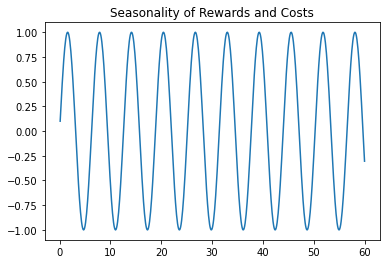
\includegraphics[width=5cm]{Figs/Seasonality.png}
            \label{fig:seasonality}
        \end{figure}
    \end{itemize}
    \end{block} 
    
\end{frame}

%%%%%%%%%%%%%%%%%%%%%%%%%%%%%%%%%%%%%%%%%%%%%%%%%%%%%%%%%%%%%

\begin{frame}{Replikator Dynamic mit periodischen Komponenten}
    \begin{block}{V=v*A*sin(x) C=1.5 (constant)}
    \begin{itemize}
        \begin{figure}[htp]
            \centering
            \begin{subfigure}
                \centering
                \includegraphics[width=0.4\textwidth]{Figs/HDSeasonal.png}
                \label{fig:HDSeasonal}
            \end{subfigure}
            \hfill
            \begin{subfigure}
                \centering
                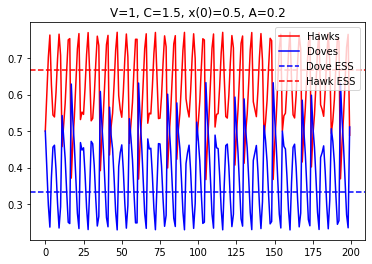
\includegraphics[width=0.4\textwidth]{Figs/HDseasonal2.png}
                \label{fig:HDSeasonal2}
            \end{subfigure}
            \hfill
        \end{figure}
    \end{itemize}
    \end{block} 
    
\end{frame}

%%%%%%%%%%%%%%%%%%%%%%%%%%%%%%%%%%%%%%%%%%%%%%%%%%%%%%%%%%%%%

\begin{frame}{Zufällige Fluktuation}
    \begin{block}{}
    \begin{itemize}
        \item Die zufällige Komponente der Replikator Dynamik wurde mithilfe eines Randomwalks mit  Elementen $\epsilon_t$ erreicht.
        \item Die Summe dieser Elemente wurde auf die periodische Payoff $V_S$ adddiert um einen stochastischen Prozess zu modellieren
        \item Die endgültige Formel für die Payoff lautet: $V_t = V_S + \sum_{n=1}^{t} \epsilon_t$
    \end{itemize}
    \end{block} 
    
\end{frame}

%%%%%%%%%%%%%%%%%%%%%%%%%%%%%%%%%%%%%%%%%%%%%%%%%%%%%%%%%%%%%

\begin{frame}{Fluktuationen}
    \begin{block}{Fluktuation der einzelnen Komponenten}
    \begin{itemize}
    \item Mithilfe dieser Formel können nun die einzelnen Komponenten berechnet werden: \pause
    \begin{figure}[htp]
            \centering
            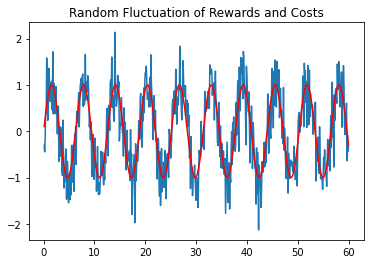
\includegraphics[width=5cm]{RFluc.png}
            \label{fig:randomfluctuation}
        \end{figure}
    \end{itemize}
    \end{block} 
    
\end{frame}

%%%%%%%%%%%%%%%%%%%%%%%%%%%%%%%%%%%%%%%%%%%%%%%%%%%%%%%%%%%%%

\begin{frame}{Replikator Dynamik mit zufälligem Payoff}
    \begin{block}{V=1 (Konstant) C streut zufällig}
    \begin{itemize}
        \begin{figure}[htp]
            \centering
            \includegraphics[width=5cm]{Konstant.png}
            \label{fig:finalpot}
        \end{figure}
    \end{itemize}
    \end{block} 
    
\end{frame}

%%%%%%%%%%%%%%%%%%%%%%%%%%%%%%%%%%%%%%%%%%%%%%%%%%%%%%%%%%%%%

\begin{frame}{Probleme mit zufälliger Streuung der Komponenten}
    \begin{alertblock}{Negative Werte}
    \begin{itemize}
        \item Die Summe der Elemente des Randomwalks können negativ sein, dies führt zu Ergebnissen die im Kontext keinen Sinn ergeben.
    \end{itemize}
    \end{alertblock} \pause
    
     \begin{block}{Lösung aus dem Paper}
    \begin{itemize}
        \item Um dieses Problem zu lösen wurde eine Hintergrund Fitness $b$ in die Replikator Gleichung eingesetzt. 
        $x_t = x_t_-_1 \cdot \frac{M \cdot \vec{x}{} +b}{\vec{x}{} \cdot M \cdot \vec{x}{} +b}$
        \item Wird ein hoher Wert für $b$ gewählt werden die negativen Einflüsse des Radomwalks kompensiert.
    \end{itemize}
    \end{block} 
\end{frame}

%%%%%%%%%%%%%%%%%%%%%%%%%%%%%%%%%%%%%%%%%%%%%%%%%%%%%%%%%%%%%

\begin{frame}{Replikator Dynamic mit periodischen Komponenten und Hintergrund Fittness}
    \begin{block}{V=v*A*sin(x) C=1.5 (constant)}
    \begin{itemize}
        \begin{figure}[htp]
            \centering
            \begin{subfigure}
                \centering
                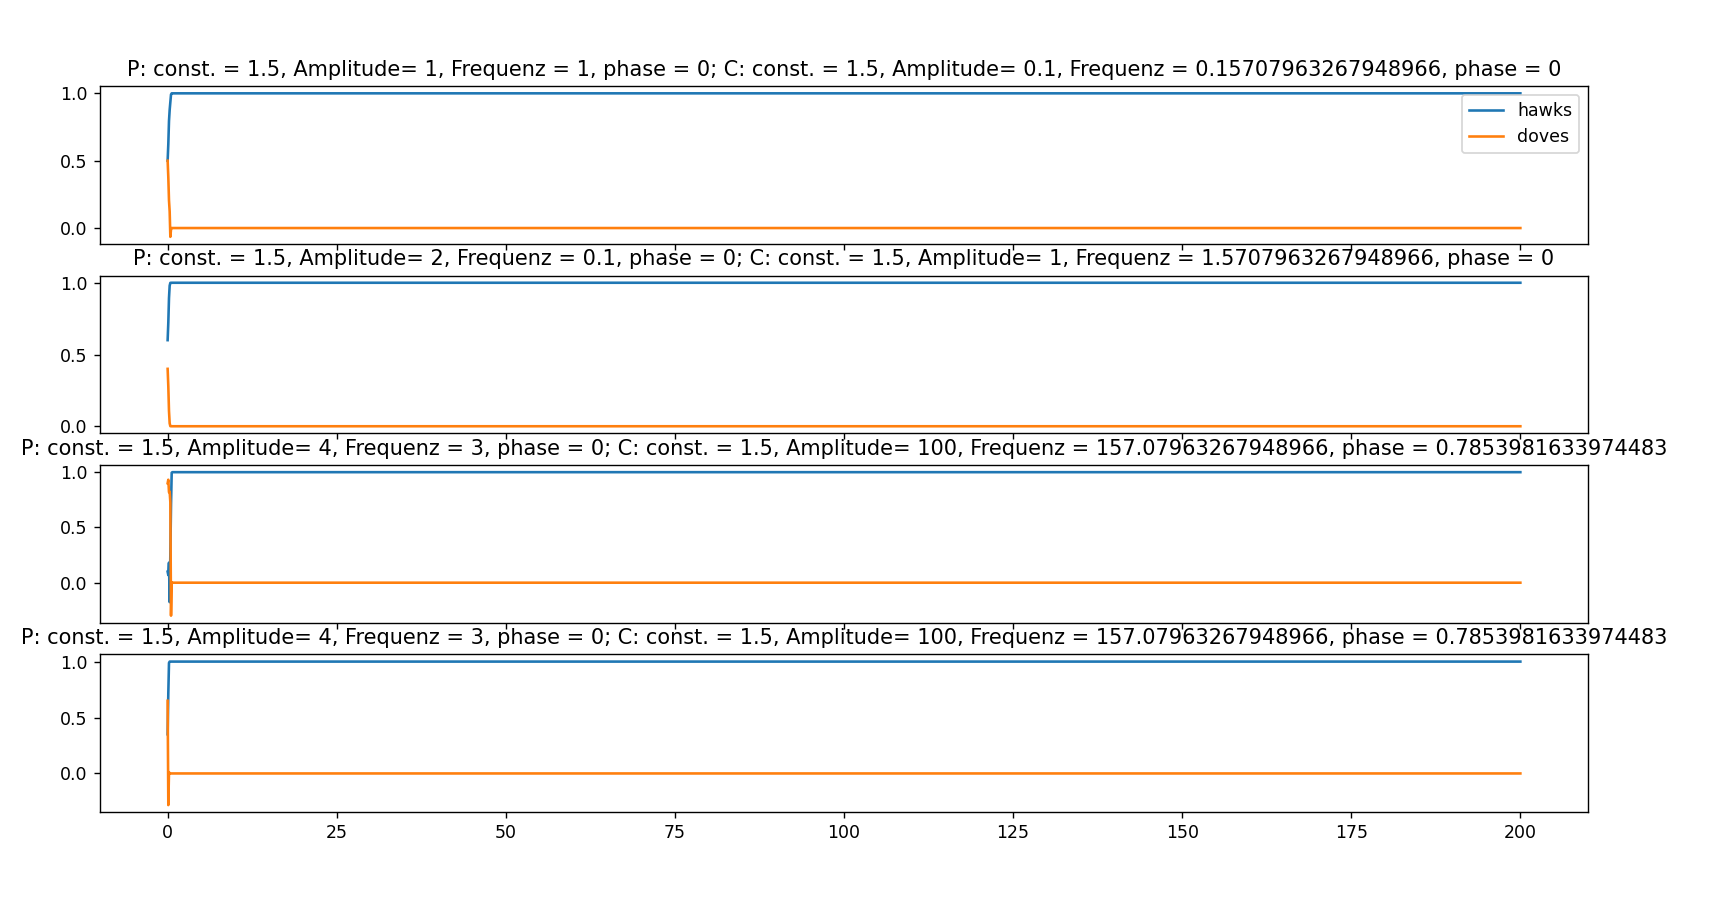
\includegraphics[width=5cm]{Figs/ohne_b.png}
                \label{fig:}
            \end{subfigure}
            \hfill
            \begin{subfigure}
                \centering
                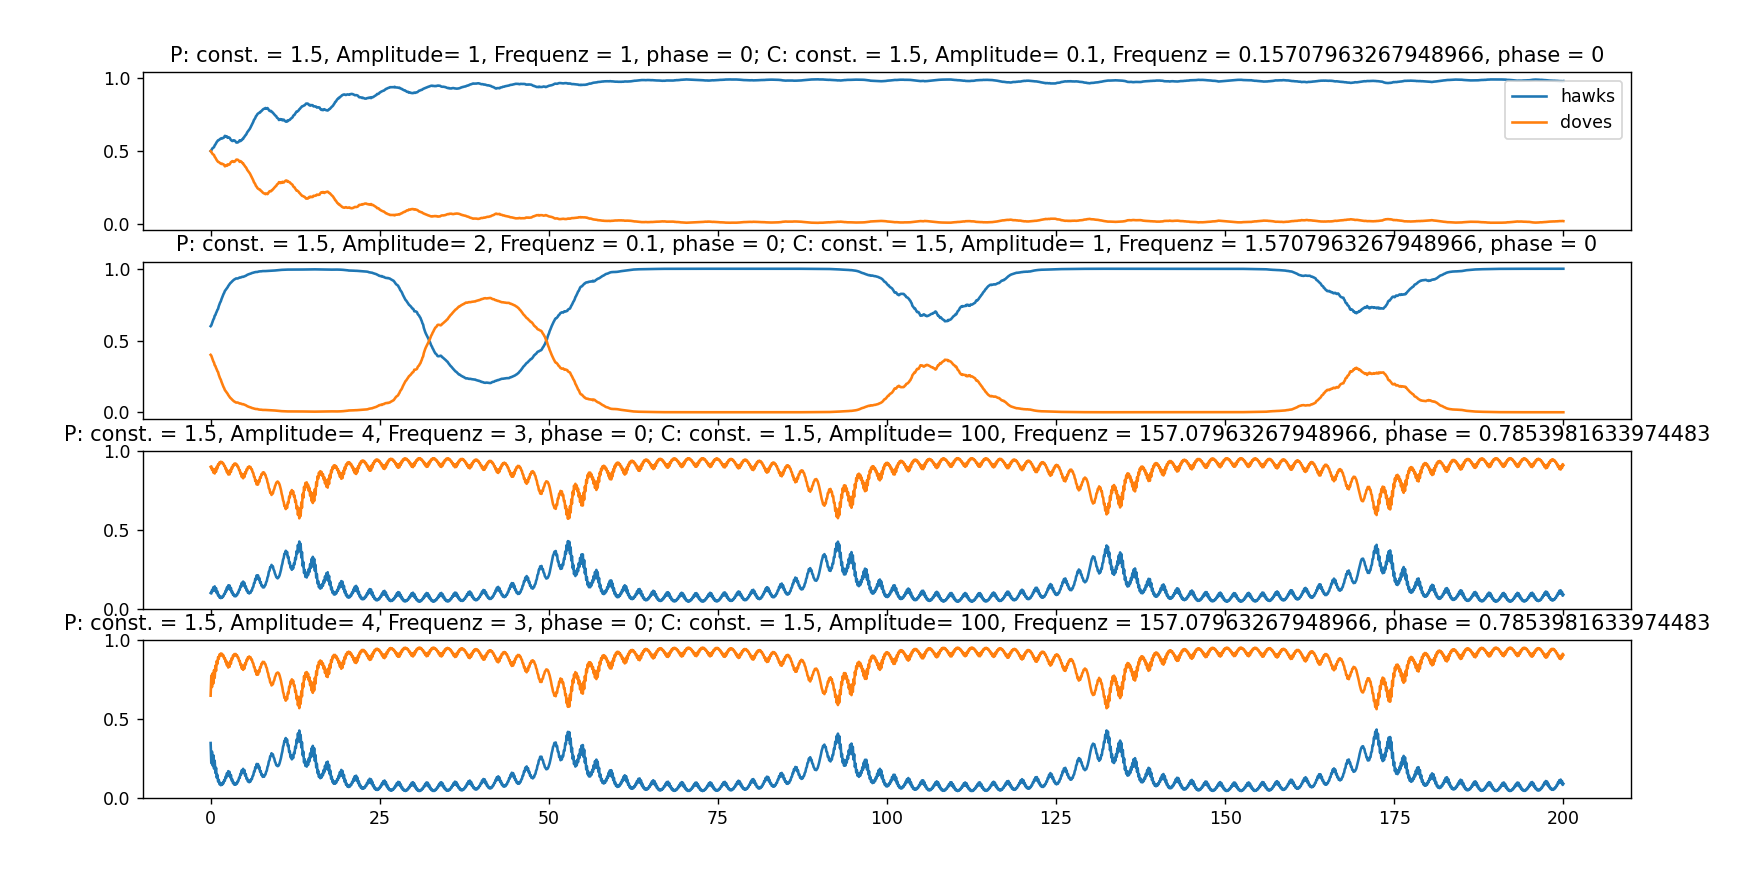
\includegraphics[width=5cm]{Figs/b.png}
                \label{fig:}
            \end{subfigure}
            \hfill
        \end{figure}
    \end{itemize}
    \end{block} 
\end{frame}






















      \begin{frame}{Zusammenfassung}
    \begin{block}{Proof of Concept}
    \begin{itemize}
        \item Modellierbarkeit einer spieltheoretischen Betrachtung
        \item Unter Verwendung: einer Payoff-Matrix und der Replikatordynamik
    \end{itemize}
    \end{block} \pause
\end{frame}

\begin{frame}{Zusamenfassung}
    \begin{block}{Bisher gesehen:}
    \begin{itemize}
        \item Vorhersehbare Entwicklung bei einfachen Systemen (Nash-Equilibrium)
        \item Interessante Entwicklung des Systems bei Fluktuationen der Parameter der Payoff-Matrix
    \end{itemize}
    \end{block}
    
\end{frame}

\begin{frame}{Ausblick}
    An verschiedenen Stellen Potenzial für interessante Betrachtungen
    \begin{block}{Fluktuation der Parameter}
    
    \begin{itemize}
        \item Welchen Einfluss haben verschiedene Formen von Fluktuationen der Parameter auf das Modell?
        \item Wie/Wann/Warum treten diese in Erscheinung?
    \end{itemize}
    \end{block}
    
\end{frame}

\begin{frame}{Ausblick}
    An verschiedenen Stellen Potenzial für interessante Betrachtungen
    \begin{block}{Fluktuation der Parameter}
    
    \begin{itemize}
        \item Welchen Einfluss haben verschiedene Formen von Fluktuationen der Parameter auf das Modell?
        \item Wie/Wann/Warum treten diese in Erscheinung?
    \end{itemize}
    \end{block}
    
    \begin{block}{Chaos?}
    \begin{itemize}
        \item Wie lassen sich bei Fluktuation der Parameter stabile Zustände herauslesen oder definieren? 
        \item Wie Ändert sich die Verlauf des Systems bei kleinen Änderungen von Entwicklungsparametern?
    \end{itemize}
    \end{block}
\end{frame}

\begin{frame}{Netzwerktheorie}
    \begin{figure}
        \centering
        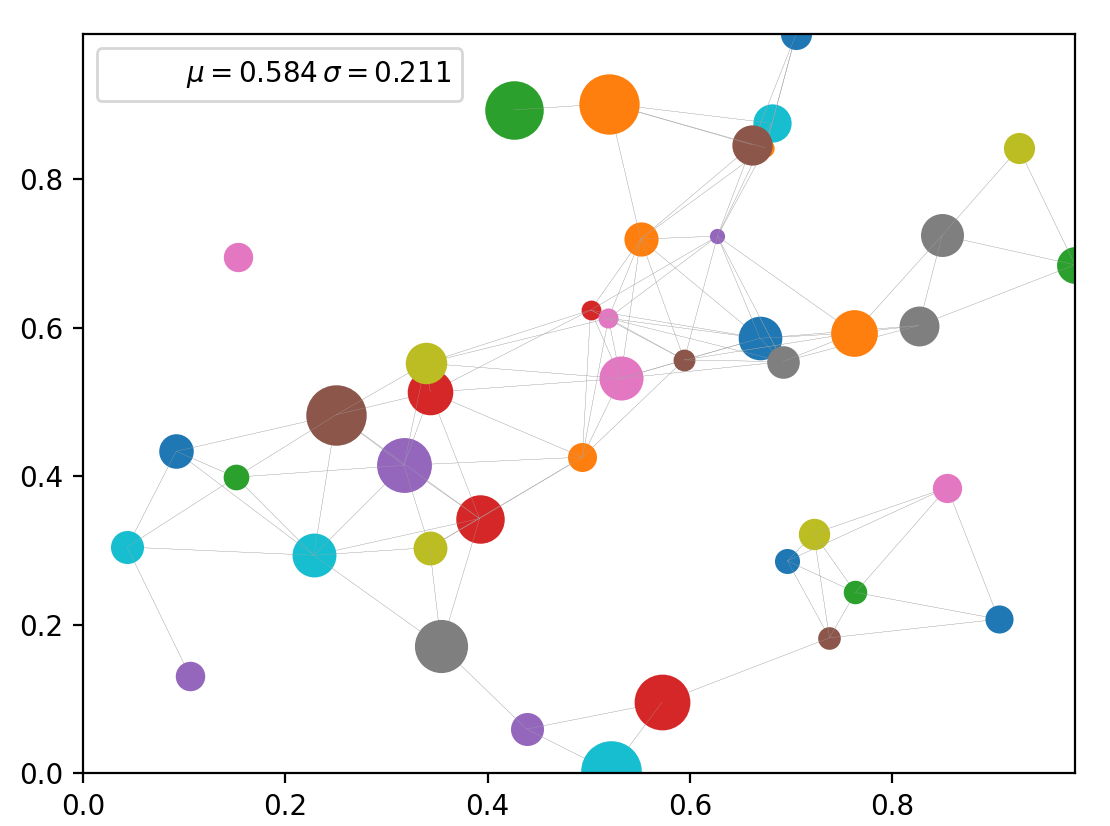
\includegraphics[width=0.7\textwidth]{Figs/Screenshot.png}
        \label{fig:my_label}
    \end{figure}
\end{frame}

\begin{frame}{Netzwerktheorie}
    \begin{block}{Migration}
    \begin{itemize}
        \item Migration zwischen Habitaten
        \item räumliche Unterschiede der Payoff-Matrix
        \item \textbf{Modellierung von demographischen Entwicklungen? Zugvogel-Verhalten?}
    \end{itemize}
    
    \end{block}
\end{frame}




%%%%%%%%%%%%%%%%%%%%%%%%%%%%%%%%%%%%%%%%%%%%%%%%%%%%%%%%%%%%%











\end{document}

